% PRD flow chart 1: the three pieces of the second-order source and where each is solved.
\documentclass[tikz,border=2pt]{standalone}
\usepackage[T1]{fontenc}
\usepackage{lmodern}
\usepackage{amsmath,amssymb}
\usetikzlibrary{arrows.meta,calc}
\newcommand{\PP}{\Phi^{\rm P}}
\newcommand{\Pres}{\Phi^{\rm res}}
\begin{document}
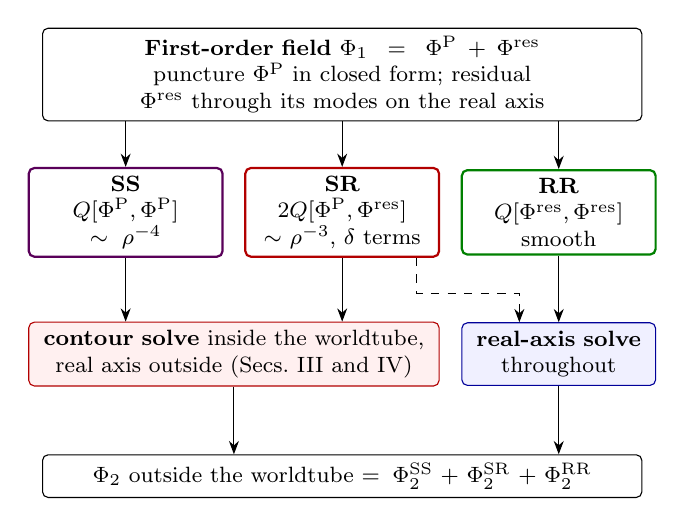
\begin{tikzpicture}[>=Stealth, font=\footnotesize,
  box/.style={draw, rounded corners=2pt, align=center, inner sep=3pt, text width=#1, fill=white}]
\node[box=7.4cm] (top) at (0,0)
  {\textbf{First-order field} $\Phi_1=\PP+\Pres$\\puncture $\PP$ in closed form; residual $\Pres$ through its modes on the real axis};
\node[box=2.25cm, draw=violet!70!black, thick] (ss) at (-2.75,-1.75)
  {\textbf{SS}\\$Q[\PP,\PP]$\\$\sim\rho^{-4}$};
\node[box=2.25cm, draw=red!70!black, thick] (sr) at (0,-1.75)
  {\textbf{SR}\\$2Q[\PP,\Pres]$\\$\sim\rho^{-3}$, $\delta$ terms};
\node[box=2.25cm, draw=green!50!black, thick] (rr) at (2.75,-1.75)
  {\textbf{RR}\\$Q[\Pres,\Pres]$\\smooth};
\node[box=5.0cm, draw=red!70!black, fill=red!6] (con) at (-1.375,-3.55)
  {\textbf{contour solve} inside the worldtube,\\real axis outside (Secs.~III and IV)};
\node[box=2.25cm, draw=blue!60!black, fill=blue!6] (real) at (2.75,-3.55)
  {\textbf{real-axis solve}\\throughout};
\node[box=7.4cm] (out) at (0,-5.1)
  {$\Phi_2$ outside the worldtube $=\Phi_2^{\rm SS}+\Phi_2^{\rm SR}+\Phi_2^{\rm RR}$};
\draw[->] (top.south -| ss) -- (ss.north);
\draw[->] (top.south) -- (sr.north);
\draw[->] (top.south -| rr) -- (rr.north);
\draw[->] (ss.south) -- (ss.south |- con.north);
\draw[->] (sr.south) -- (sr.south |- con.north);
\draw[->, dashed] ($(sr.south east)+(-0.3,0)$) -- ++(0,-0.45) -| ($(real.north)+(-0.5,0)$);
\draw[->] (rr.south) -- (real.north);
\draw[->] (con.south) -- (con.south |- out.north);
\draw[->] (real.south) -- (real.south |- out.north);
\end{tikzpicture}
\end{document}
